\documentclass[a4paper,12 pt,oneside]{report}     % Type de document
\usepackage[utf8x]{inputenc}			  % Utilisation du UTF8
\usepackage{textcomp}				  % Accents dans les titres
\usepackage [ french ] {babel}                    % Titres en français
\usepackage [T1] {fontenc} 			  % Correspondance clavier -> document
\usepackage[Lenny]{fncychap}                      % Beau Chapitre
\usepackage{dsfont}                    	  % Pour afficher N,Z,D,Q,R,C
\usepackage{fancyhdr}                             % Entete et pied de pages
\usepackage [outerbars] {changebar}               % Positionnement barre en marge externe
\usepackage{amsmath}				  % Utilisation de la librairie de Maths
%\usepackage{amsfont}				  % Utilisation des polices de Maths
\usepackage{cite}                                 % Citations de la bibliographie
\usepackage{openbib}                              % Gestion avancée de Bibtex
\usepackage{enumerate}				  % Permet d'utiliser la fonction énumerate
\usepackage{dsfont}				  % Utilisation des polices Dsfont
\usepackage{ae}					  % Rend le PDF plus lisible
\usepackage[pdftex]{graphicx}
\usepackage{graphics}

\newtheorem{de}{Définition}
\newtheorem{theo}{Théorème}
\newtheorem{enon}{Énoncé}
\newtheorem{prop}{Propriété}
%opening
\title{Amplificateurs opérationnels}
\author{MP}
\begin{document}
\maketitle
\tableofcontents
\chapter{Les montages usuels}
\section{Amplificateur inverseur}
\subsection{Schéma}
\begin{figure}[!h]
  \centering
  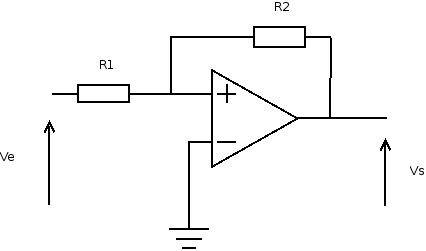
\includegraphics[width=5cm]{ampliopinverseur.png}
  \caption{Amplificateur inverseur}
\end{figure}
\subsection{Sortie}
$$ V_\mathrm{s} = - V_\mathrm{e} \left ( \dfrac{R_\mathrm{2}}{R_\mathrm{1}} \right)$$
\section{Amplificateur non-inverseur}
\subsection{Schéma}
\begin{figure}
  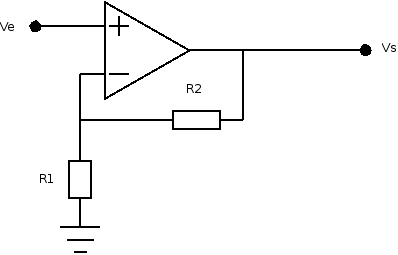
\includegraphics{ampliopnoninverseur.png}
  \caption{Amplificateur non-inverseur}
\end{figure}

\end{document}
